%%%%
\teteTermStssDosa

%%%% titre
\vspace*{-30pt}
\numeroActivite{2}
\titreTP{Analyse sanguine}
\vspace*{-4pt}


%%%% objectifs
\begin{objectifs}
  \item Comprendre le principe d'un dosage spectrophotométrique.
  \item Interpréter les résultats d'une analyse sanguine.
  \item Réaliser un dosage par étalonnage.
\end{objectifs}

\begin{contexte}
  Pour vérifier son état de santé, on effectue souvent des analyses de sang, qui représentent \qty{90}{\percent} des analyses médicales.
  
  Le sang est une solution composé d'un liquide (le plasma), de cellules (plaquettes, globules rouges et blancs) et d'un grand nombre d'espèces chimiques.
  
  \problematique{
    Comment mesurer la concentration en hémoglobine dans un échantillon sanguin ?
  }
\end{contexte}


%%%%
\begin{doc}{Principe de la spectrophotométrie}{doc:TP2_spectro}
  Pour déterminer la concentration d'une solution en hémoglobine, on peut utiliser une \important{courbe d'étalonnage} obtenue par \important{spectrophotométrie.}

  Un spectrophotomètre mesure \important{l'absorbance $A$} d'une espèce chimique colorée en solution pour une longueur d'onde $\lambda$ donnée.
  La longueur d'onde est choisie pour avoir \important{une absorbance maximale.}
  L'absorbance est une grandeur sans unité qui est \important{proportionnelle} à la concentration de l'espèce colorée étudiée.
\end{doc}

\question{
  Quelles est la relation mathématique qui lie deux grandeurs proportionnelles ?
  Graphiquement, comment peut-on observer que deux grandeurs sont proportionnelles ?
}{}{3}


\begin{doc}{Principe du dosage par étalonnage de l'hémoglobine}{doc:TP2_dosage_hb}
  \begin{wrapfigure}[10]{r}{0.6\linewidth}
    \centering
    \vspace*{-18pt}
    \image{1}{images/donnees/absorbance_hemoglobine}
  \end{wrapfigure}
  
  L'hémoglobine est responsable de la teinte rouge du sang.
  Cette coloration du sang est proportionnelle à la quantité d'hémoglobine présente dans le sang.
  L'absorbance est donc proportionnelle à la quantité d'hémoglobine dans le sang.
  
  Ci-contre, des courbes d'absorbance pour différentes \important{solutions étalons} avec des concentrations d'hémoglobine connues ont été mesurées.
  
  C'est le principe du \important{dosage par étalonnage} : on mesure l'absorbance d'une gamme de solutions étalons avec différentes concentrations pour obtenir une droite d'étalonnage.
  En  mesurant l'absorbance de l'échantillon de sang que l'on veut doser, on peut donc déterminer la concentration en hémoglobine en réalisant une simple lecture graphique.
\end{doc}

\question{
  Pour quelle valeur de la longueur d'onde l'absorbance est-elle maximale ?
}{}{1}

\mesure Tracer la concentration en hémoglobine en fonction de l'absorbance maximale.

\question{
  Après utilisation du spectrophotomètre sur l'échantillon de sang d'un patient, on trouve une absorbance de 1,1 pour \qty{430}{\nm}.
  Donner, en justifiant, la concentration en hémoglobine du patient.
}{}{3}


%%%%
\begin{doc}{Résultats d'analyse}{doc:TP2_resultat_analyse}
  L'analyse sanguine complète du patient est donné ci-dessous :
  \begin{boite}
  \textbf{LABORATOIRES BioTech} \hfill
  \textbf{Patient : A. Coulibaly}

  \vspace*{-12pt}
  \begin{center}
    \begin{tblr}{
      colspec = {l l l },
    }
      & \important{Résultats de l'analyse} & \important{Valeurs de référence} \\
      %
      \important{Hématologie} & & \\
      Leucocytes & \textbf{\qty{4,19}{G\per\litre}} & 1,50 à \qty{4,00}{G\per\litre} \\
      Hémoglobine & \qty{14,5}{\g\per\deci\litre} &  à \qty{}{\g\per\deci\litre} \\
      Plaquettes & \qty{301}{G\per\litre} & 150 à \qty{300}{G\per\litre} \\
      %
      \important{Bilan lipidique} & & \\
      Triglycérides & \textbf{\qty{1,80}{\g\per\litre}} & < \qty{1,50}{\g\per\litre} \\
      Cholestérol total & \textbf{\qty{2,50}{\g\per\litre}} & < \qty{2}{\g\per\litre} \\
       %
      \important{Chimie du sang} & & \\
       Glycémie à jeun & \qty{0,811}{\milli\g\per\litre} & 0,70 à \qty{1,10}{\g\per\litre} \\
       Ferritine & \qty{118,3}{\milli\g\per\litre} & 22,0 à \qty{322,0}{\g\per\litre} \\
    \end{tblr}
  \end{center}
  * \unit{G\per\litre} : milliard de cellule par litre.
  \end{boite}
\end{doc}

\question{
  Est-ce que le résultat de l'analyse pour l'hémoglobine est cohérent avec ce que vous avez mesuré à partir de la courbe d'étalonnage ?
}{}{3}


\begin{doc}{Bilan lipidique}{doc:TP2_lipidique}
  Le bilan lipidique indique les taux en cholestérol total et en triglycérides.
  Des valeurs trop élevées en cholestérol sont des facteurs à risque pour les maladies cardio-vasculaires.

  Une modification du régime alimentaire peut permettre de réduire son taux de cholestérol, en diminuant les graisses saturées ou « trans » et en augmentant la consommation de fibres alimentaire ou d'oméga 3.
\end{doc}

\begin{doc}{Glycémie}{doc:TP2_glycemie}
  La glycémie à jeun correspond à la concentration en glucose dans le sang après un minimum de 12 heures de jeûne.

  Une glycémie à jeun inférieur à \qty{1,09}{\g\per\litre} révèle un état non-diabétique.
  De 1,10 à \qty{1,25}{\g\per\litre}, c'est le signe d'une mauvaise tolérance au glucose.
  Une valeur supérieure ou égale à \qty{1,26}{\g\per\litre} obtenue lors de deux analyses successives indique que le ou la patiente souffre de diabète.

  Une trop grand concentration de glucose dans le sang entraine des dégâts dans l'ensemble du corps (yeux, reins, système cardiaque, etc.).
\end{doc}

%%
\question{
  Indiquer la concentration en triglycérides de M. Coulibaly
}{
}{1}

\question{
  Le corps d'un homme adulte contient environ \qty{5}{\litre} de sang.
  Calculer la concentration massique en triglycéride de M. Coulibaly.
}{
}{2}

\question{
  Tracer un axe horizontal et indiquer les trois zones décrites dans le document~\ref{doc:TP2_glycemie}.
}{
}{3}

\question{
  Interpréter les résultats d'analyse de M. Coulibaly et indiquer quels conseils nutritionnels il devrait suivre.
}{}{4}

\includepdf[pages=26]{commun/papier_millimetre}